% Options for packages loaded elsewhere
\PassOptionsToPackage{unicode}{hyperref}
\PassOptionsToPackage{hyphens}{url}
\PassOptionsToPackage{dvipsnames,svgnames,x11names}{xcolor}
%
\documentclass[
]{article}

\usepackage{amsmath,amssymb}
\usepackage{iftex}
\ifPDFTeX
  \usepackage[T1]{fontenc}
  \usepackage[utf8]{inputenc}
  \usepackage{textcomp} % provide euro and other symbols
\else % if luatex or xetex
  \usepackage{unicode-math}
  \defaultfontfeatures{Scale=MatchLowercase}
  \defaultfontfeatures[\rmfamily]{Ligatures=TeX,Scale=1}
\fi
\usepackage{lmodern}
\ifPDFTeX\else  
    % xetex/luatex font selection
\fi
% Use upquote if available, for straight quotes in verbatim environments
\IfFileExists{upquote.sty}{\usepackage{upquote}}{}
\IfFileExists{microtype.sty}{% use microtype if available
  \usepackage[]{microtype}
  \UseMicrotypeSet[protrusion]{basicmath} % disable protrusion for tt fonts
}{}
\makeatletter
\@ifundefined{KOMAClassName}{% if non-KOMA class
  \IfFileExists{parskip.sty}{%
    \usepackage{parskip}
  }{% else
    \setlength{\parindent}{0pt}
    \setlength{\parskip}{6pt plus 2pt minus 1pt}}
}{% if KOMA class
  \KOMAoptions{parskip=half}}
\makeatother
\usepackage{xcolor}
\usepackage[lmargin=1in,rmargin=1in,tmargin=1in,bmargin=1in]{geometry}
\setlength{\emergencystretch}{3em} % prevent overfull lines
\setcounter{secnumdepth}{3}
% Make \paragraph and \subparagraph free-standing
\ifx\paragraph\undefined\else
  \let\oldparagraph\paragraph
  \renewcommand{\paragraph}[1]{\oldparagraph{#1}\mbox{}}
\fi
\ifx\subparagraph\undefined\else
  \let\oldsubparagraph\subparagraph
  \renewcommand{\subparagraph}[1]{\oldsubparagraph{#1}\mbox{}}
\fi

\providecommand{\tightlist}{%
  \setlength{\itemsep}{0pt}\setlength{\parskip}{0pt}}\usepackage{longtable,booktabs,array}
\usepackage{calc} % for calculating minipage widths
% Correct order of tables after \paragraph or \subparagraph
\usepackage{etoolbox}
\makeatletter
\patchcmd\longtable{\par}{\if@noskipsec\mbox{}\fi\par}{}{}
\makeatother
% Allow footnotes in longtable head/foot
\IfFileExists{footnotehyper.sty}{\usepackage{footnotehyper}}{\usepackage{footnote}}
\makesavenoteenv{longtable}
\usepackage{graphicx}
\makeatletter
\def\maxwidth{\ifdim\Gin@nat@width>\linewidth\linewidth\else\Gin@nat@width\fi}
\def\maxheight{\ifdim\Gin@nat@height>\textheight\textheight\else\Gin@nat@height\fi}
\makeatother
% Scale images if necessary, so that they will not overflow the page
% margins by default, and it is still possible to overwrite the defaults
% using explicit options in \includegraphics[width, height, ...]{}
\setkeys{Gin}{width=\maxwidth,height=\maxheight,keepaspectratio}
% Set default figure placement to htbp
\makeatletter
\def\fps@figure{htbp}
\makeatother
% definitions for citeproc citations
\NewDocumentCommand\citeproctext{}{}
\NewDocumentCommand\citeproc{mm}{%
  \begingroup\def\citeproctext{#2}\cite{#1}\endgroup}
\makeatletter
 % allow citations to break across lines
 \let\@cite@ofmt\@firstofone
 % avoid brackets around text for \cite:
 \def\@biblabel#1{}
 \def\@cite#1#2{{#1\if@tempswa , #2\fi}}
\makeatother
\newlength{\cslhangindent}
\setlength{\cslhangindent}{1.5em}
\newlength{\csllabelwidth}
\setlength{\csllabelwidth}{3em}
\newenvironment{CSLReferences}[2] % #1 hanging-indent, #2 entry-spacing
 {\begin{list}{}{%
  \setlength{\itemindent}{0pt}
  \setlength{\leftmargin}{0pt}
  \setlength{\parsep}{0pt}
  % turn on hanging indent if param 1 is 1
  \ifodd #1
   \setlength{\leftmargin}{\cslhangindent}
   \setlength{\itemindent}{-1\cslhangindent}
  \fi
  % set entry spacing
  \setlength{\itemsep}{#2\baselineskip}}}
 {\end{list}}
\usepackage{calc}
\newcommand{\CSLBlock}[1]{\hfill\break\parbox[t]{\linewidth}{\strut\ignorespaces#1\strut}}
\newcommand{\CSLLeftMargin}[1]{\parbox[t]{\csllabelwidth}{\strut#1\strut}}
\newcommand{\CSLRightInline}[1]{\parbox[t]{\linewidth - \csllabelwidth}{\strut#1\strut}}
\newcommand{\CSLIndent}[1]{\hspace{\cslhangindent}#1}

\usepackage{float}
\makeatletter
\@ifpackageloaded{caption}{}{\usepackage{caption}}
\AtBeginDocument{%
\ifdefined\contentsname
  \renewcommand*\contentsname{Table of contents}
\else
  \newcommand\contentsname{Table of contents}
\fi
\ifdefined\listfigurename
  \renewcommand*\listfigurename{List of Figures}
\else
  \newcommand\listfigurename{List of Figures}
\fi
\ifdefined\listtablename
  \renewcommand*\listtablename{List of Tables}
\else
  \newcommand\listtablename{List of Tables}
\fi
\ifdefined\figurename
  \renewcommand*\figurename{Figure}
\else
  \newcommand\figurename{Figure}
\fi
\ifdefined\tablename
  \renewcommand*\tablename{Table}
\else
  \newcommand\tablename{Table}
\fi
}
\@ifpackageloaded{float}{}{\usepackage{float}}
\floatstyle{ruled}
\@ifundefined{c@chapter}{\newfloat{codelisting}{h}{lop}}{\newfloat{codelisting}{h}{lop}[chapter]}
\floatname{codelisting}{Listing}
\newcommand*\listoflistings{\listof{codelisting}{List of Listings}}
\makeatother
\makeatletter
\makeatother
\makeatletter
\@ifpackageloaded{caption}{}{\usepackage{caption}}
\@ifpackageloaded{subcaption}{}{\usepackage{subcaption}}
\makeatother

\usepackage{hyphenat}
\usepackage{ifthen}
\usepackage{calc}
\usepackage{calculator}


\usepackage{geometry}

\usepackage{graphicx}
\usepackage{geometry}
\usepackage{afterpage}
\usepackage{tikz}
\usetikzlibrary{calc}
\usetikzlibrary{fadings}
\usepackage[pagecolor=none]{pagecolor}


% Set the titlepage font families







% Set the coverpage font families

\ifLuaTeX
  \usepackage{selnolig}  % disable illegal ligatures
\fi
\IfFileExists{bookmark.sty}{\usepackage{bookmark}}{\usepackage{hyperref}}
\IfFileExists{xurl.sty}{\usepackage{xurl}}{} % add URL line breaks if available
\urlstyle{same} % disable monospaced font for URLs
\hypersetup{
  pdftitle={Scale-freeness and Growth Stability of Realistic Network Models},
  pdfauthor={Thomas Boughen},
  colorlinks=true,
  linkcolor={blue},
  filecolor={Maroon},
  citecolor={Blue},
  urlcolor={Blue},
  pdfcreator={LaTeX via pandoc}}

\title{Scale-freeness and Growth Stability of Realistic Network Models}
\usepackage{etoolbox}
\makeatletter
\providecommand{\subtitle}[1]{% add subtitle to \maketitle
  \apptocmd{\@title}{\par {\large #1 \par}}{}{}
}
\makeatother
\subtitle{Project Approval}
\author{Thomas Boughen}
\date{}

\begin{document}
%%%%% begin titlepage extension code


\begin{titlepage}

%%% TITLE PAGE START

% Set up alignment commands
%Page
\newcommand{\titlepagepagealign}{
\ifthenelse{\equal{center}{right}}{\raggedleft}{}
\ifthenelse{\equal{center}{center}}{\centering}{}
\ifthenelse{\equal{center}{left}}{\raggedright}{}
}


\newcommand{\titleandsubtitle}{
% Title and subtitle
{{\Huge{\textbf{\nohyphens{Scale-freeness and Growth Stability of
Realistic Network Models}}}}\par
}%

\vspace{\betweentitlesubtitle}
{
{\LARGE{\nohyphens{Project Approval}}}\par
}}
\newcommand{\titlepagetitleblock}{
\titleandsubtitle
}

\newcommand{\authorstyle}[1]{{\textbf{#1}}}

\newcommand{\affiliationstyle}[1]{{\large{#1}}}

\newcommand{\titlepageauthorblock}{
{\authorstyle{\nohyphens{Thomas Boughen}\\}}
}

\newcommand{\titlepageaffiliationblock}{
\hangindent=1em
\hangafter=1
{\affiliationstyle{


\vspace{1\baselineskip} 
}}
}
\newcommand{\headerstyled}{%
{}
}
\newcommand{\footerstyled}{%
{\Large{\textsc{Newcastle University 2023}}}
}
\newcommand{\datestyled}{%
{}
}


\newcommand{\titlepageheaderblock}{\headerstyled}

\newcommand{\titlepagefooterblock}{
\footerstyled
}

\newcommand{\titlepagedateblock}{
\datestyled
}

%set up blocks so user can specify order
\newcommand{\titleblock}{\newlength{\betweentitlesubtitle}
\setlength{\betweentitlesubtitle}{0.5cm}
{

{\titlepagetitleblock}
}

\vspace{1.5cm}
}

\newcommand{\authorblock}{{\titlepageauthorblock}

\vspace{2\baselineskip}
}

\newcommand{\affiliationblock}{{\titlepageaffiliationblock}

\vspace{1pt}
}

\newcommand{\logoblock}{{\includegraphics[width=1in]{University\_of\_Newcastle\_Coat\_of\_Arms.png}}

\vspace{1cm}
}

\newcommand{\footerblock}{{\titlepagefooterblock}

\vspace{1pt}
}

\newcommand{\dateblock}{}

\newcommand{\headerblock}{}
\newgeometry{top=3in,bottom=1in,right=0.3in,left=0.3in}

\thispagestyle{empty} % no page numbers on titlepages


\newlength{\minipagewidth}
\setlength{\minipagewidth}{\textwidth}
\raggedright % single minipage
% [position of box][box height][inner position]{width}
% [s] means stretch out vertically; assuming there is a vfill
\begin{minipage}[b][\textheight][s]{\minipagewidth}
\titlepagepagealign
\titleblock

\authorblock

\vfill

\logoblock

\footerblock
\par

\end{minipage}\ifthenelse{\equal{}{right} \OR \equal{}{leftright} }{
\hspace{\B}
\vrulecode}{}
\clearpage
\restoregeometry
%%% TITLE PAGE END
\end{titlepage}
\setcounter{page}{1}

%%%%% end titlepage extension code
\section{Research Proposal}\label{research-proposal}

\subsection{Background}\label{sec-bg}

Networks often arise when representing complex systems and the
relationships between the components within them. Take a social network
such as X (formerly Twitter) as an example, new users can join at any
time and ``follow'' other users so that they can keep up with their
posts. This forms a directed network where each user corresponds to a
node and there exists an edge going from one users node to another if
the former ``follows'' the latter. The number of ``followers'' of any
one user is therefore the in-degree of the corresponding node in the
network, is a quantity of interest when it comes to analysing how the
network and each node's in-degree may grow in the future. This is just
one example of a network, others include:

\begin{itemize}
\item
  The Facebook friends of Harvard students and alumni
\item
  Interactions between proteins in cells
\item
  Game results between tennis players
\item
  Dependencies of R packages
\end{itemize}

The survival functions of the degrees of nodes in each of these networks
are shown below in Figure~\ref{fig-survs}.

\begin{figure}[H]

\centering{

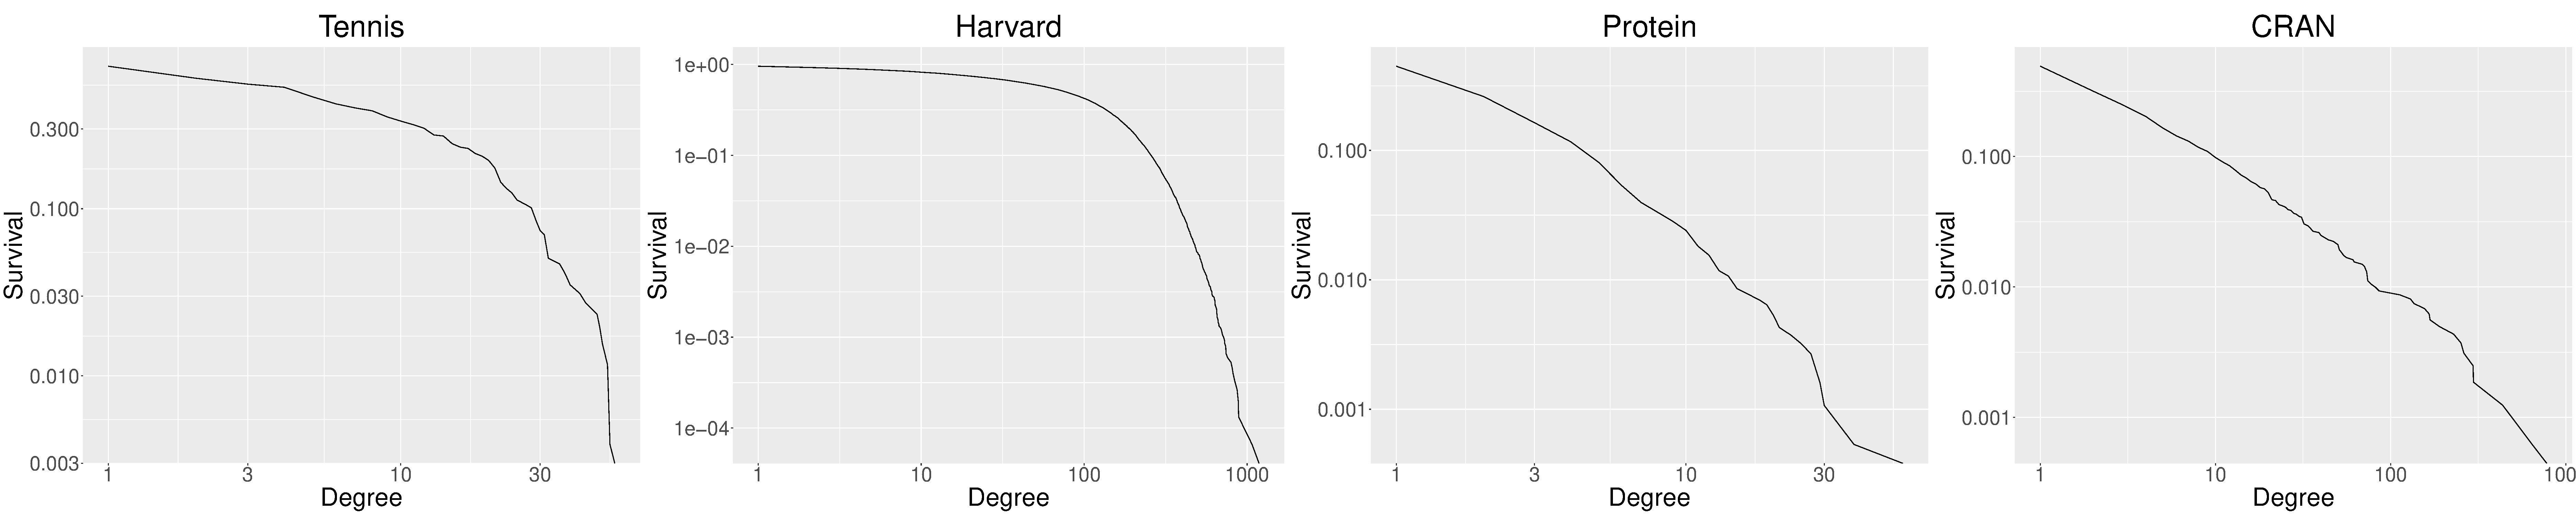
\includegraphics[width=0.9\textwidth,height=\textheight]{proposal_files/figure-pdf/fig-survs-1.pdf}

}

\caption{\label{fig-survs}Survival function of the degrees.}

\end{figure}%

The variety of fields across which networks appear make them a vital
source of data to be able to analyse, there is particular interest in
the way that the networks might have grown. Network generative models
describe the way in which nodes and edges are added and removed from
networks over time. One might naively propose that nodes in a network
are connected to other nodes independently with equal probability, this
gives rise to the Random Network Model (Gilbert 1959) which has been
proven to generate a network that has a binomial degree distribution
which looks nothing like the degree distribution of a lot of real
networks. This isn't the only property where this model does not
accurately represent real networks. One attempt to create a more
accurate network generative model comes from (Barabási and Albert 1999)
who noted that the number of nodes in a network grows over time and that
nodes tend to connect to the other nodes in the network with more
connections (preferential attachment).

\subsubsection{Barabási-Albert model}\label{barabuxe1si-albert-model}

They proposed a minimal model called the Barabási-Albert model, also
known as the BA model, which is defined below:

Start with \(m_0\) nodes , the edges between them chosen arbitrarily
such that each node has at least one link. The network then develops
using two steps:

\begin{enumerate}
\def\labelenumi{\arabic{enumi}.}
\item
  Growth

  At each time step, add a node to the network that will connect to
  \(m\le m_0\) nodes (already in the network) with \(m\) edges.
\item
  Preferential Attachment

  The probability that an edge from the new node connects to node \(i\)
  is proportional to its current degree \(k_i\) i.e \(k_i/\sum_{j}k_j\).
\end{enumerate}

This model generates a network with an approximate power law degree
distribution, which looks a lot closer to the degree distributions of
real networks and is very simple. Therefore when analysing a network it
is tempting to say that it has a power law degree distribution so the BA
model can be used to model its growth. The survival function of the
degrees of a network produced following this scheme is shown in
Figure~\ref{fig-surv-sim}.

\begin{figure}[H]

\centering{

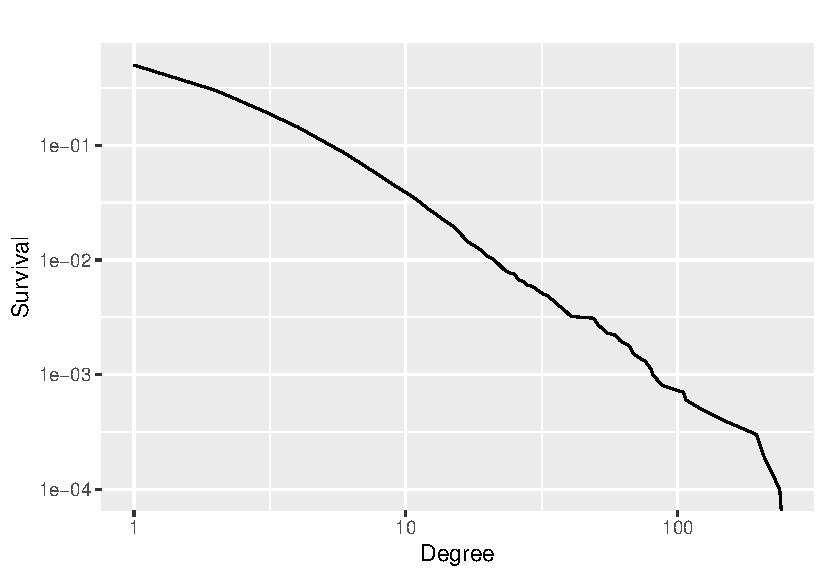
\includegraphics[width=0.9\textwidth,height=\textheight]{proposal_files/figure-pdf/fig-surv-sim-1.pdf}

}

\caption{\label{fig-surv-sim}Survival function of the degrees for data
simulated under BA model.}

\end{figure}%

This does look quite similar to some of the plots in
Figure~\ref{fig-survs} like the CRAN data and protein interactions, but
looks very different to the some of the others.

According to recent works (Broido and Clauset 2019; Voitalov et al.
2019) real networks have more nuanced degree distributions and the power
law, while suitable for the bulk of the data, is inadequate for the full
set of degrees. This is especially clear in the right tail and, to a
lesser extent, the left tail. Despite this, methods from extreme value
theory remain underutilised even though they seem well suited to the
problem of modelling the tails of the degree distribution.

\subsection{Aims}\label{aims}

This brings us to the aims of this project, which is to firstly find a
suitable model for the degree distribution of real networks using
methods from extreme value theory, such as a threshold model where the
majority of the degrees are modeled by power laws and the right tail is
modeled using a discretised version of the Generalised Pareto
distribution, the Integer Generalised Pareto distribution (IGP). Then
after finding a suitable model for the degree distribution, measuring
the changes in model parameters over time for real networks. Informing
the modification and/or extension of the BA model to generate networks
with the desired degree distribution, such that the new model
satisfactorily explains how real networks might have grown. The
theoretical properties of networks generated by this model can then be
studied, for example how close to following a power law is the networks
degree distribution and how do the largest degrees in the network change
over time.

\subsection{Methodology}\label{methodology}

As mentioned in the previous subsection, we begin by trying to find a
suitable model for the degree distribution of real networks.

\subsubsection{Power Law Model}\label{sec-pl}

We first look at the power law distribution and fit it to the degree
distributions of some real networks using a Bayesian approach.

The power law model is characterised by only one parameter
\(\alpha\in\mathbb{R}^+\) and has probability mass function (PMF):

\[
f(x) = \frac{x^{-(\alpha+1)}}{\zeta(\alpha+1)}, \qquad x=1,2,\ldots
\]

where \(\zeta(\alpha+1) = \sum_{k=1}^\infty k^{-(\alpha+1)}\) is the
Riemann Zeta function.

A good visual tool for judging the fit of the model is the survival
function which we define below:

\[
S(x) = 1 - \frac{\sum_{k=1}^x k^{-(\alpha+1)}}{\zeta(\alpha+1)}, \qquad x=1,2,\ldots
\]

\paragraph{Bayesian Inferenece for the Power Law
model}\label{bayesian-inferenece-for-the-power-law-model}

We aim to fit this model using a Bayesian approach and as such we need
to define the likelihood for a set of degrees
\(\boldsymbol{x} = (x_1, x_2, \ldots, x_N)^T\). We introduce the
auxilliary variables \(\boldsymbol{y} = (y_1, y_2, \ldots y_m)^T\) and
\(\boldsymbol{c} = (c_1, c_2, \ldots,c_m)^T\) to be the unique values of
\(x_i \in \boldsymbol{x}\) and the counts of these unique values in the
vector \(\boldsymbol{x}\) respectively, with the constraint that
\(N = \sum_{i=1}^m c_i\). This is to align the formation of the
likelihood with those of the coming models as it will lead to more
efficient computations. That said, we now define the likelihood below:

\[
L(\boldsymbol{x}) = L(\boldsymbol{y},\boldsymbol{c}) =  \zeta(\alpha+1)^{-N}\prod_{i=1}^m y_i^{-c_i(\alpha+1)}
\] Now that we have the likelihood, in order to continue with the
Bayesian method we need to decide on a prior for \(\alpha\), we choose
an uninformative prior of \(\alpha\sim Ga(1,\lambda_\alpha)\) for an
adequately small \(\lambda_\alpha\in\mathbb{R^+}\). This gives us the
posterior distribution of:

\[
\pi(\alpha|\boldsymbol{x}) \propto \lambda_\alpha e^{-\alpha\lambda_\alpha}\zeta(\alpha+1)^{-N}\prod_{i=1}^m y_i^{-c_i(\alpha+1)}
\] The results of fitting this model to various data sets are shown in
Section~\ref{sec-wsf}.

\subsubsection{Power Law Mixture}\label{sec-plpl}

Before we can introduce the power law IGP mixture, we would like a model
that we can use to benchmark it against. To that end, we look at a
mixture of two power laws which seems natural to use as there does seem
to be a change in gradient in some of the plots in
Figure~\ref{fig-survs}.

This model uses a right truncated power law with exponent \(\alpha+1\)
for the bulk of the data and then a left truncated power law with
exponent \(\beta+1\) for the remainder.

The PMF of this model is defined below: \[
f(x) = \begin{cases}
(1-\phi)\frac{x^{-(\alpha+1)}}{\sum_{k=1}^v k^{-(\alpha+1)}}, &x=1,2,\ldots v\\
\phi\frac{x^{-(\beta+1)}}{\zeta(\beta+1, v+1)}, &x=v+1,v+2,\ldots
\end{cases}
\] where \(v=\lceil u\rceil\) for some \(u\in\mathbb{R}^+\),
\(\alpha\in\mathbb{R}\), \(\beta\in\mathbb{R}^+\), \(\phi\in(0,1)\) and
\(\zeta(\beta+1, v+1) = \sum_{k=v+1}^\infty k^{-(\beta+1)}\) is the
Hurwitz Zeta function\footnote{Note that \(\alpha\) can now be any real
  number, since the model is right truncated and therefore the
  denominator of the probability mass function will converge for any
  real \(\alpha\). \(\beta\) is more restricted since the denominator of
  the corresponding probability mass function is an infinite sum and
  therefore does not converge for \(\beta \le 0\)}.

The survival function is fairly simple to calculate:

\[
S(x) = \begin{cases}
(1-\phi)\left[1-\frac{\sum_{k=1}^x k^{-(\alpha+1)}}{\sum_{k=1}^v k^{-(\alpha+1)}}\right],&x=1,2,\ldots,v \\
\phi\left[1-\frac{\sum_{k=v+1}^x k^{-(\beta+1)}}{\zeta(\beta+1, v+1)}\right],&x=v+1,v+2,\ldots
\end{cases}
\]

\paragraph{Bayesian Inferenece for the Power Law Mixture
Model}\label{bayesian-inferenece-for-the-power-law-mixture-model}

We again calculate the likelihood using the auxiliary variables
\(\boldsymbol{y}\) and \(\boldsymbol{c}\): \[
L(\boldsymbol{x}) = (1-\phi)^n\phi^{N-n}\zeta(\beta+1, v+1)^{n-N}\left(\sum_{k=1}^v k^{-(\alpha+1)}\right)^{-n}\prod_{i:y_i\le v}y_i^{-c_i(\alpha+1)}\prod_{i:y_i>v}y_i^{-c_i(\beta+1)}
\] We now specify the priors used to calculate the posterior
distribution:

\begin{align*}
\alpha &\sim N(0,1/\lambda_\alpha)\\
\beta &\sim Ga(1,\lambda_\beta)\\
\phi &\sim Beta(1,1)
\end{align*}

These are all relatively uninformative priors for any adequately small
values of \(\lambda_\alpha\) and \(\lambda_\beta\). We do not decide on
a prior for \(u\) directly, instead choosing to specify it through
\(\phi\).

We now continue to calculate the posterior distribution:

\begin{align*}
\pi(\alpha, \beta, u|\boldsymbol{x}) \propto &\lambda_\alpha^{-1}\lambda_\beta\exp\{-(\beta\lambda_\beta + \alpha^2\lambda_\alpha)\}\zeta(\beta+1, v+1)^{n-N}\left(\sum_{k=1}^v k^{-(\alpha+1)}\right)^{-n}\\&\times\prod_{i:y_i\le v}y_i^{-c_i(\alpha+1)}\prod_{i:y_i>v}y_i^{-c_i(\beta+1)}
%
\end{align*}

We fit this model for the same sets of data as we did for the previous
models and the results are show next in Section~\ref{sec-wsf}.

\subsubsection{Power Law IGP Mixture Model (PL-IGP)}\label{sec-pli}

To define this model we will first need to look at a traditional way of
modelling extreme values, more specifically approximating the
conditional distribution of the largest values. This is often done using
the Generalised Pareto distribution (GPD) is parameter by the scale
parameter \(\sigma\in \mathbb{R}^+\), the shape parameter
\(\xi \in \mathbb{R}\) ,and a threshold \(u\in \mathbb{R}^+\). It is
denoted by \(Y|Y>u \sim GPD(\sigma,\xi)\) where \(Y\) is some continuous
random variable. The GPD has survival function defined below:

\[
\Pr(Y>y|Y>u) = \left(1+\frac{\xi(y-u)}{\sigma}\right)_+^{-1/\xi}, \qquad y>u
\] where \(a_+ = \max(0,a)\).

However, this is only really appropriate to use for approximating the
conditional distribution of the largest values of continuous random
variables. So, we would like a similar distribution that can be used for
discrete random variables.

\paragraph{Integrated Generalised Pareto Distribution
(IGPD)}\label{integrated-generalised-pareto-distribution-igpd}

We follow roughly the same method as Rohrbeck et al. (2018), but they
only consider modelling \(Y=\lceil H\rceil\) we also consider the
possibility of modelling \(Y=\lfloor H\rfloor\) where \(H\) is a
continuous random variable with support on the positive real line such
the \(H|H>u \sim GPD(\sigma_0 + \xi u, \xi)\) for some
\(u\in \mathbb{R}^+\). Below we define the PMF of the IGPD for both
cases.

\subparagraph{\texorpdfstring{Ceiling Version: the case where
\(Y=\lceil H \rceil\)}{Ceiling Version: the case where Y=\textbackslash lceil H \textbackslash rceil}}\label{ceiling-version-the-case-where-ylceil-h-rceil}

For values of \(x = \lfloor u \rfloor , \lfloor u \rfloor +1, \ldots\)
and \(\xi\in\mathbb{R}\) and \(u,\sigma_0 \in \mathbb{R}^+\):

\begin{align*}
\Pr(Y=x|Y>u) &= \Pr(H<x|H>\lfloor u \rfloor) - \Pr(H<x-1|H>\lfloor u \rfloor)\\ 
             &= \left(1+\frac{\xi(x-\lfloor u \rfloor)}{\sigma_0 + \xi \lfloor u \rfloor}\right)_+^{-1/\xi} - \left(1+\frac{\xi(x-1-\lfloor u \rfloor)}{\sigma_0 + \xi \lfloor u \rfloor}\right)_+^{-1/\xi}\\
%
\end{align*}

\subparagraph{\texorpdfstring{Floor Version: the case where
\(Y=\lfloor H \rfloor\)}{Floor Version: the case where Y=\textbackslash lfloor H \textbackslash rfloor}}\label{floor-version-the-case-where-ylfloor-h-rfloor}

For values of \(x = \lceil u \rceil , \lceil u \rceil +1, \ldots\) and
\(\xi\in\mathbb{R}\) and \(u,\sigma_0 \in \mathbb{R}^+\):

\begin{align*}
\Pr(Y=x|Y>u) &= \Pr(H<x+1|H>\lceil u \rceil) - \Pr(H<x|H>\lceil u \rceil)\\ 
             &= \left(1+\frac{\xi(x+1-\lceil u \rceil)}{\sigma_0 + \xi \lceil u \rceil}\right)_+^{-1/\xi} - \left(1+\frac{\xi(x-\lceil u \rceil)}{\sigma_0 + \xi \lceil u \rceil}\right)_+^{-1/\xi}\\
%
\end{align*}

For the sake of briefness, from here on out we will always be using the
floor version of the IGPD, but note that the results can be easily
extended for the ceiling version.

This now allows us to define the mixture model of a truncated power law
and the IGPD, which has the PMF: \[
f(x) = 
\begin{cases}
(1-\phi)\frac{x^{-(\alpha+1)}}{\sum_{k=1}^v k^{-(\alpha+1)}},&x=1,2,\ldots,v\\
\phi\left[\left(1+\frac{\xi(x+1-v)}{\sigma_0 + \xi v}\right)_+^{-1/\xi} - \left(1+\frac{\xi(x-v)}{\sigma_0 + \xi v}\right)_+^{-1/\xi}\right], &x=v+1, v+2, \ldots
\end{cases}
\] For \(\phi\in(0,1)\), \(\sigma_0 \in \mathbb{R}^+\),
\(\alpha\in\mathbb{R}\), \(\xi \in (-\sigma_0/v, \infty)\)\footnote{Again
  \(\alpha\) has an extended domain due to the power law now being right
  truncated. To simplify the expressions that follow we define:}, and
\(v=\lceil u \rceil\) for \(u \in \mathbb{R}^+\).

\[
G(x) = \left(1+\frac{\xi(x-v)}{\sigma_0 + \xi v}\right)_+^{-1/\xi}
\] Again, we want the survival function so we can get an idea of how
well the model performs for real data. It is defined as:

\[
S(x) = \begin{cases}
(1-\phi)\left[1-\frac{\sum_{k=1}^xk^{-(\alpha+1)}}{\sum_{k=1}^v k^{-(\alpha+1)}}\right], &x=1,2,\ldots,v\\
\phi G(x+1),&x=v+1,v+2, \ldots
\end{cases}
\] We continue to fit this model using a Bayesian methodology, so we
define the likelihood again using the auxiliary variables
\(\boldsymbol{y}\) and \(\boldsymbol{c}\) and we obtain the below:

\[
L(\boldsymbol{x}) = L(\boldsymbol{y}, \boldsymbol{c}) = \phi^{N-n}(1-\phi)^n \left(\sum_{k=1}^v k^{-(\alpha+1)}\right)^{-n}\prod_{i:y_i\le v}y_i^{-c_i(\alpha+1)}\prod_{i:y_i>v}\left[G(y_i+1) - G(y_i)\right]^{c_i}
\] where \(n\) is the number of values in \(\boldsymbol{x}\) that are at
most \(v\).

\paragraph{Bayesian Inferenece for the PL-IGP
model}\label{bayesian-inferenece-for-the-pl-igp-model}

Proceeding with the Bayesian approach, we decide on the following priors
for the parameters:

\begin{align*}
\alpha &\sim N(0,1/\lambda_\alpha),\\
\xi &\sim N(0,1/\lambda_\xi),\\
\sigma_0 &\sim Ga(1,\lambda_\sigma),\\
\phi &\sim Beta(1,1)\\
%
\end{align*}

Again, we are using fairly uninformative priors for the parameters.
Using the same method of indirectly specifying a prior for \(u\) through
the prior of \(\phi\) instead.

With all of this we find the posterior distribution to be:

\begin{align*}
\pi(\alpha,\sigma_0, \xi, u| \boldsymbol{x}) \propto & (2\pi)^{-1}\lambda_\alpha^{1/2}\lambda_\xi^{1/2}\lambda_\sigma\exp\{-[\sigma_0\lambda_\sigma + \frac{1}{2}(\alpha^2\lambda_\alpha + \xi^2\lambda_\xi)]\} \left(\sum_{k=1}^v k^{-(\alpha+1)}\right)^{-n}\\& \times \prod_{i:y_i\le v}y_i^{-c_i(\alpha+1)}\prod_{i:y_i>v}\left[G(y_i+1) - G(y_i)\right]^{c_i}
\end{align*}

As before, the results of fitting this model to several data sets are
found in Section~\ref{sec-wsf}.

\subsection{Work So Far}\label{sec-wsf}

So far, we have started looking for a model that is adequate for
modelling the degree distributions of real networks. We have used some
adaptive Metropolis-Hastings algorithms using methods similar to those
in \emph{Handbook of Markov Chain Monte Carlo} (2011) and Xiang and Neal
(2014) to obtain estimates and credible intervals for the model
parameters. Below we show the results of this for the same data sets
shown in Figure~\ref{fig-survs}, alongside the fits to the data shown in
Figure~\ref{fig-surv-sim} which was simulated using the BA model.

\subsubsection{The Power Law}\label{the-power-law}

In Figure~\ref{fig-pl} below we can see that for some sets of data the
power law does an good job for the bulk of the data, but it doesn't fit
well in the right tail usually lying above the empirical survival curve.
For other sets of data, the model seems completely inadequate namely for
the Tennis and Harvard data sets. These results were obtained using the
prior parameter \(\lambda_\alpha = 0.01\) and an initial value of
\(\alpha=1\) in an adaptive Metropolis-Hastings algorithm for 100,000
iterations with a burn in period of 500 iterations and then thinned by
5, yielding a minimum effective sample size of 2,000.

\begin{figure}[H]

\centering{

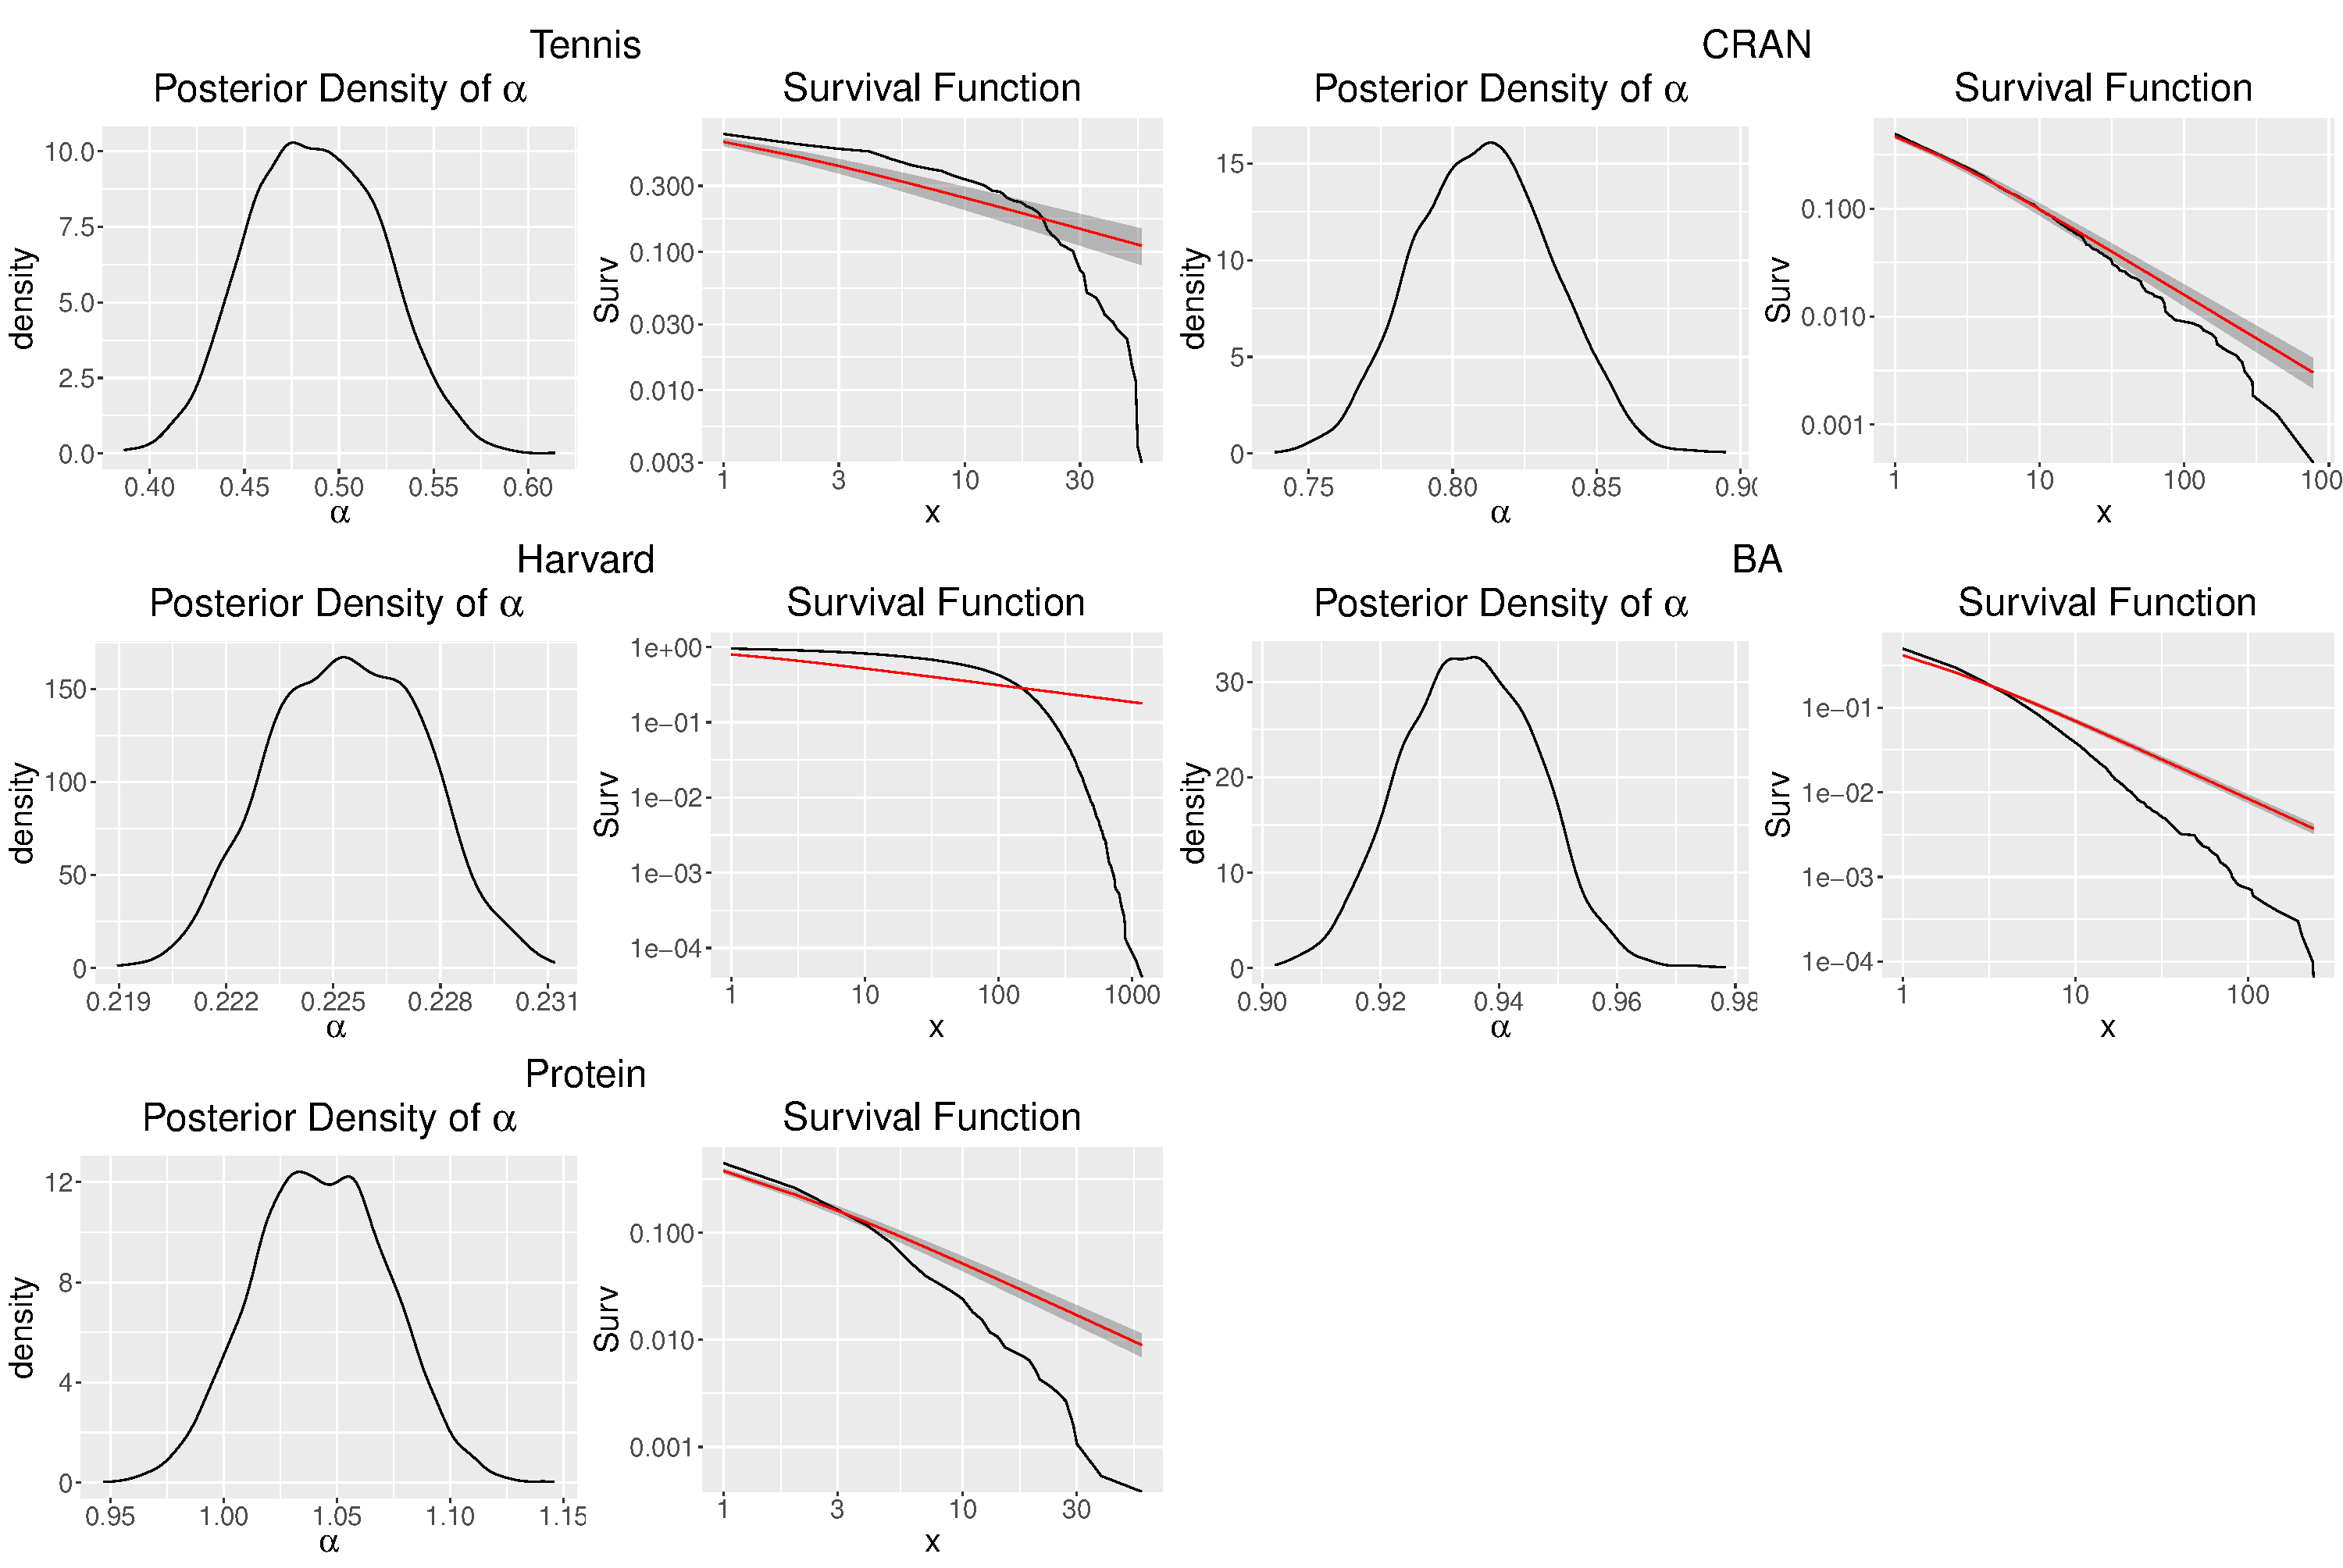
\includegraphics{proposal_files/figure-pdf/fig-pl-1.pdf}

}

\caption{\label{fig-pl}Plots of fitted survival functions and posterior
densities of \(\alpha\).}

\end{figure}%

\subsubsection{Power Law IGP Model}\label{power-law-igp-model}

This mixture model defined in Section~\ref{sec-pli} seems to perform
significantly better for all of the data sets. Within each group of
plots in Figure~\ref{fig-pli}, the posterior densities are shown for
each of the parameters and then in the bottom left of each group is the
95\% credible interval for the survival. While this model seems to fit
these sets of data well, it may be needlessly complex and have more
parameters than necessary. So, next we fit the model described in
Section~\ref{sec-plpl}.

\begin{figure}[H]

\centering{

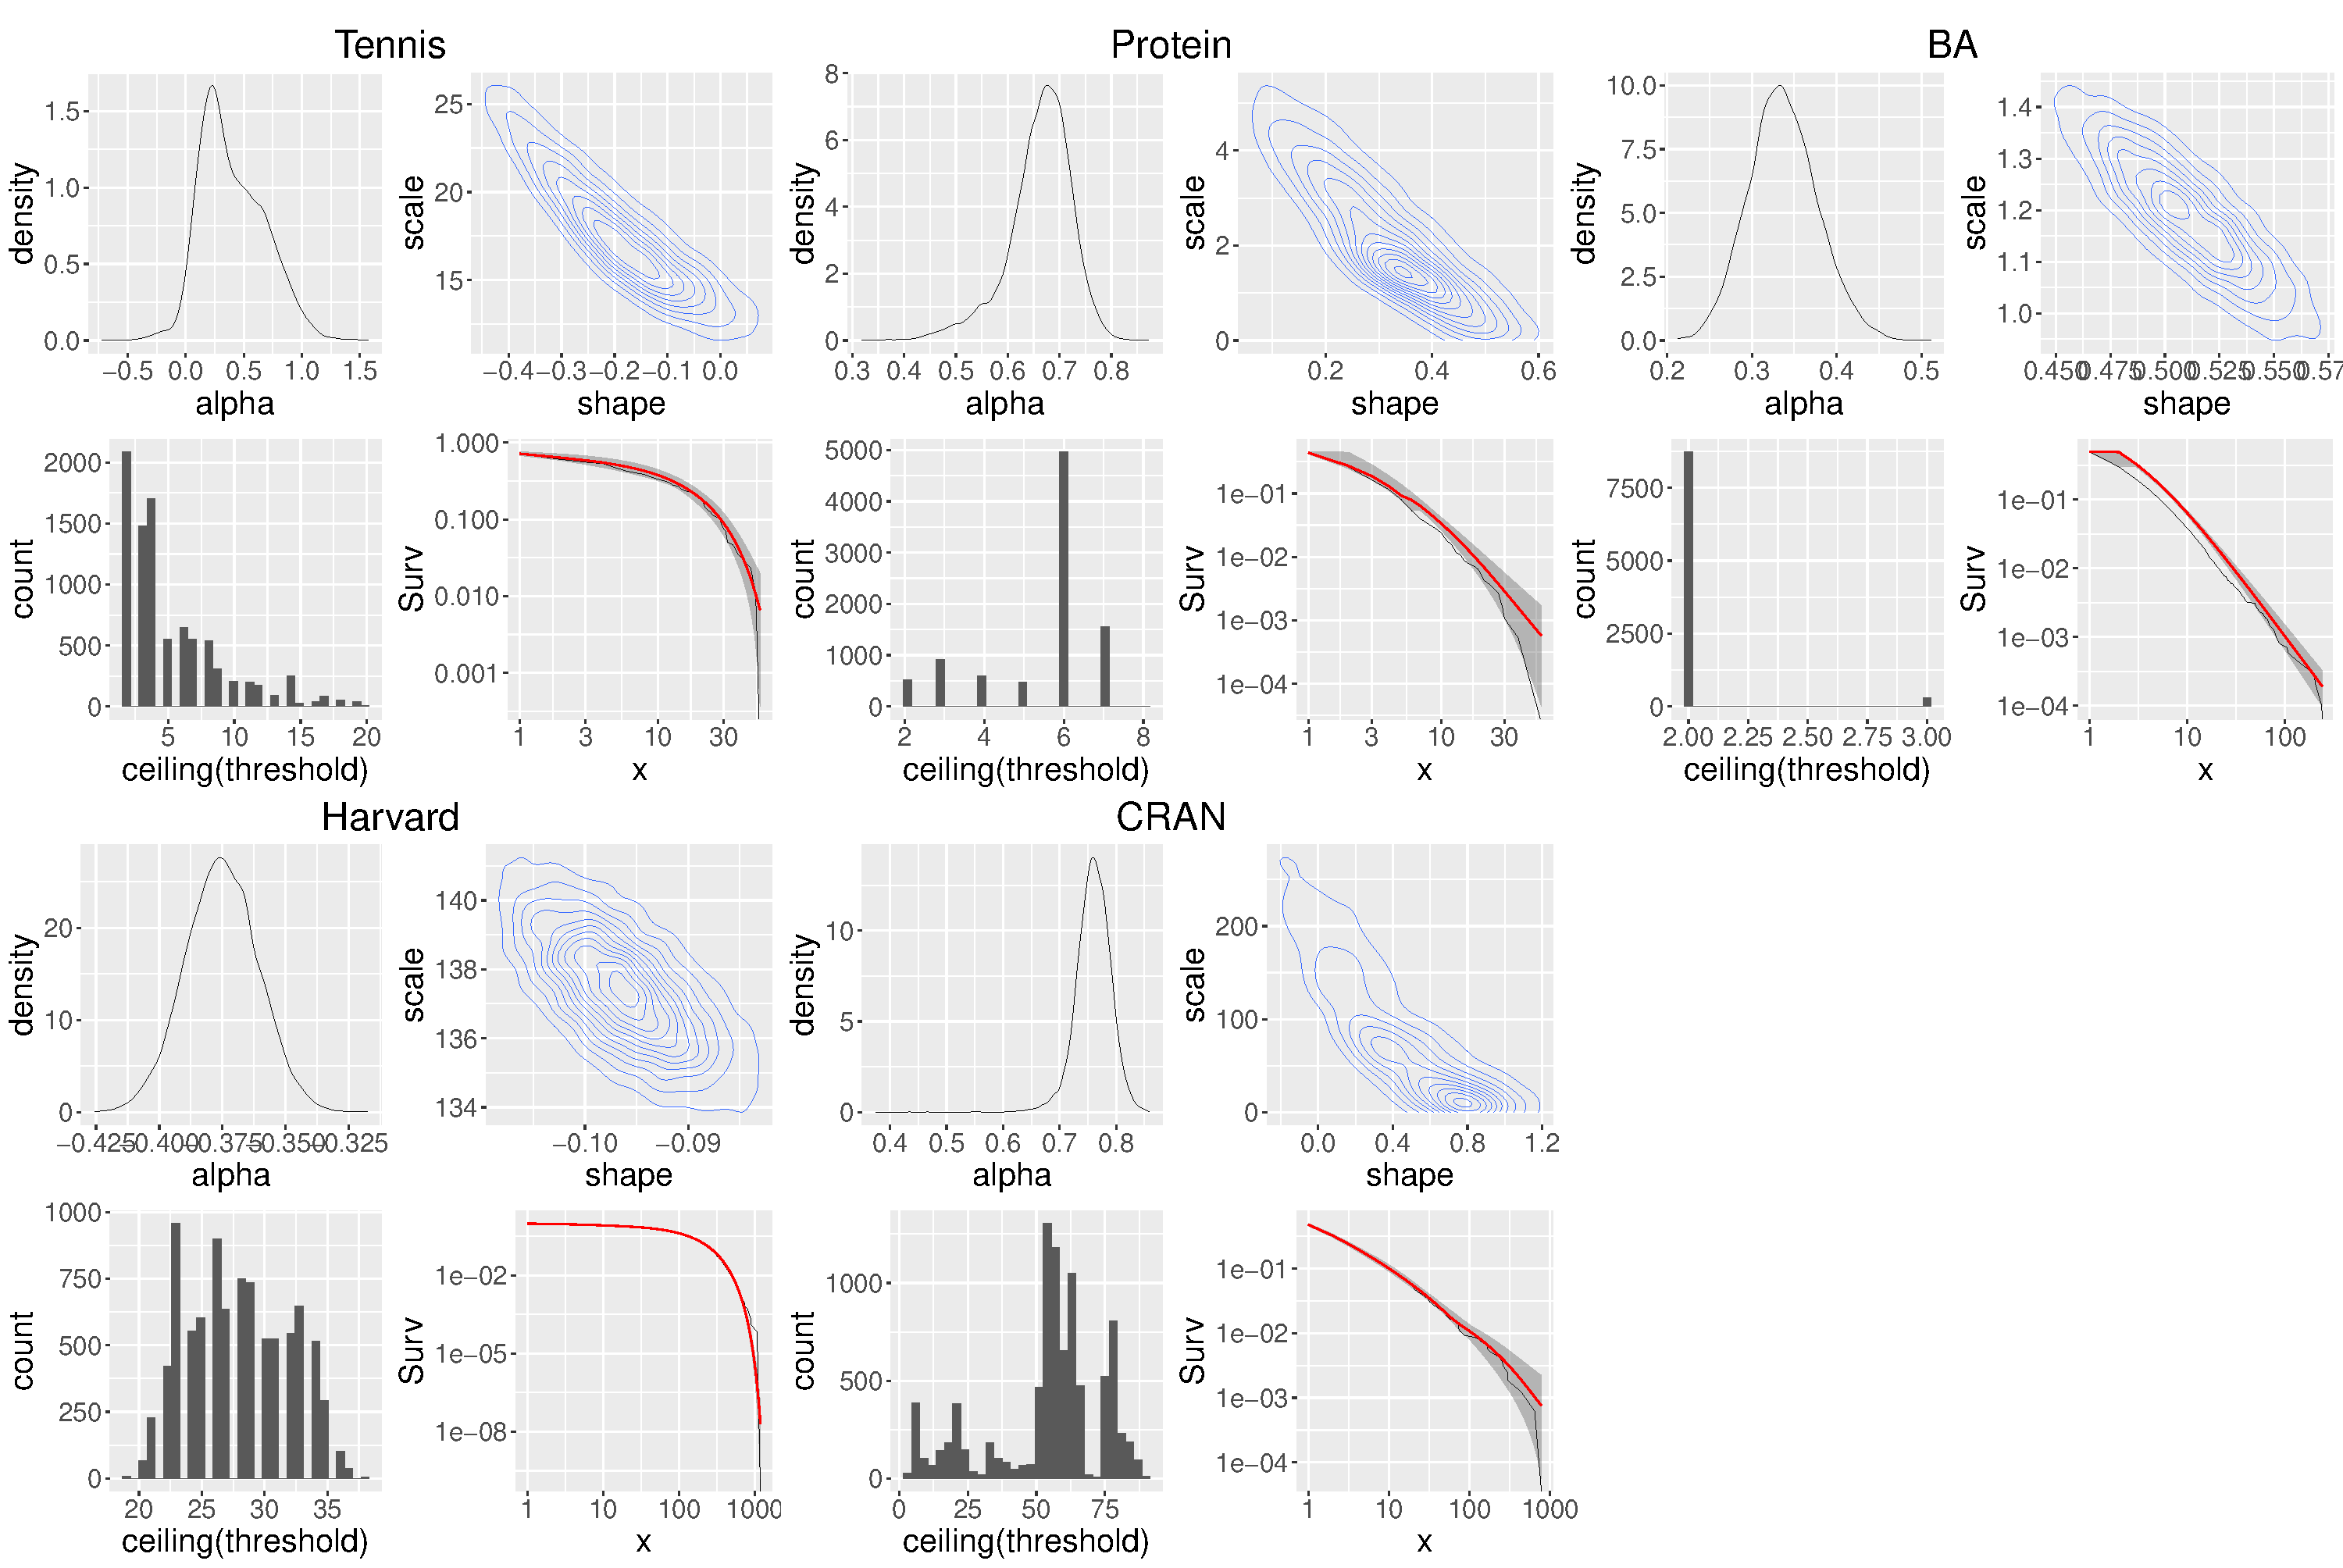
\includegraphics{proposal_files/figure-pdf/fig-pli-1.pdf}

}

\caption{\label{fig-pli}Plots of fitted survival functions and posterior
densities for the parameters.}

\end{figure}%

\subsubsection{Power Law Mixture}\label{power-law-mixture}

Looking at Figure~\ref{fig-plpl}, this model also seems to perform quite
well for all of the sets of data. In the top left of each group of plots
is a 2D density plot of the two different power law parameters,
\(\alpha\) and \(\beta\). In the top right is a histogram of the value
of \(\lceil u\rceil\) and finally, in the bottom right is a plot of the
empirical survival function with the posterior mean in red and 95\%
credible intervals for the survival. It is interesting to note that, for
the simulated data, the value of \(\lceil u \rceil\) did not stray from
the value of 3 indicating that using only one power law may be suitable
which was expected. This also happens to be the minimum value that the
code will allow the threshold to take since model selection has not been
implemented.

\begin{figure}[H]

\centering{

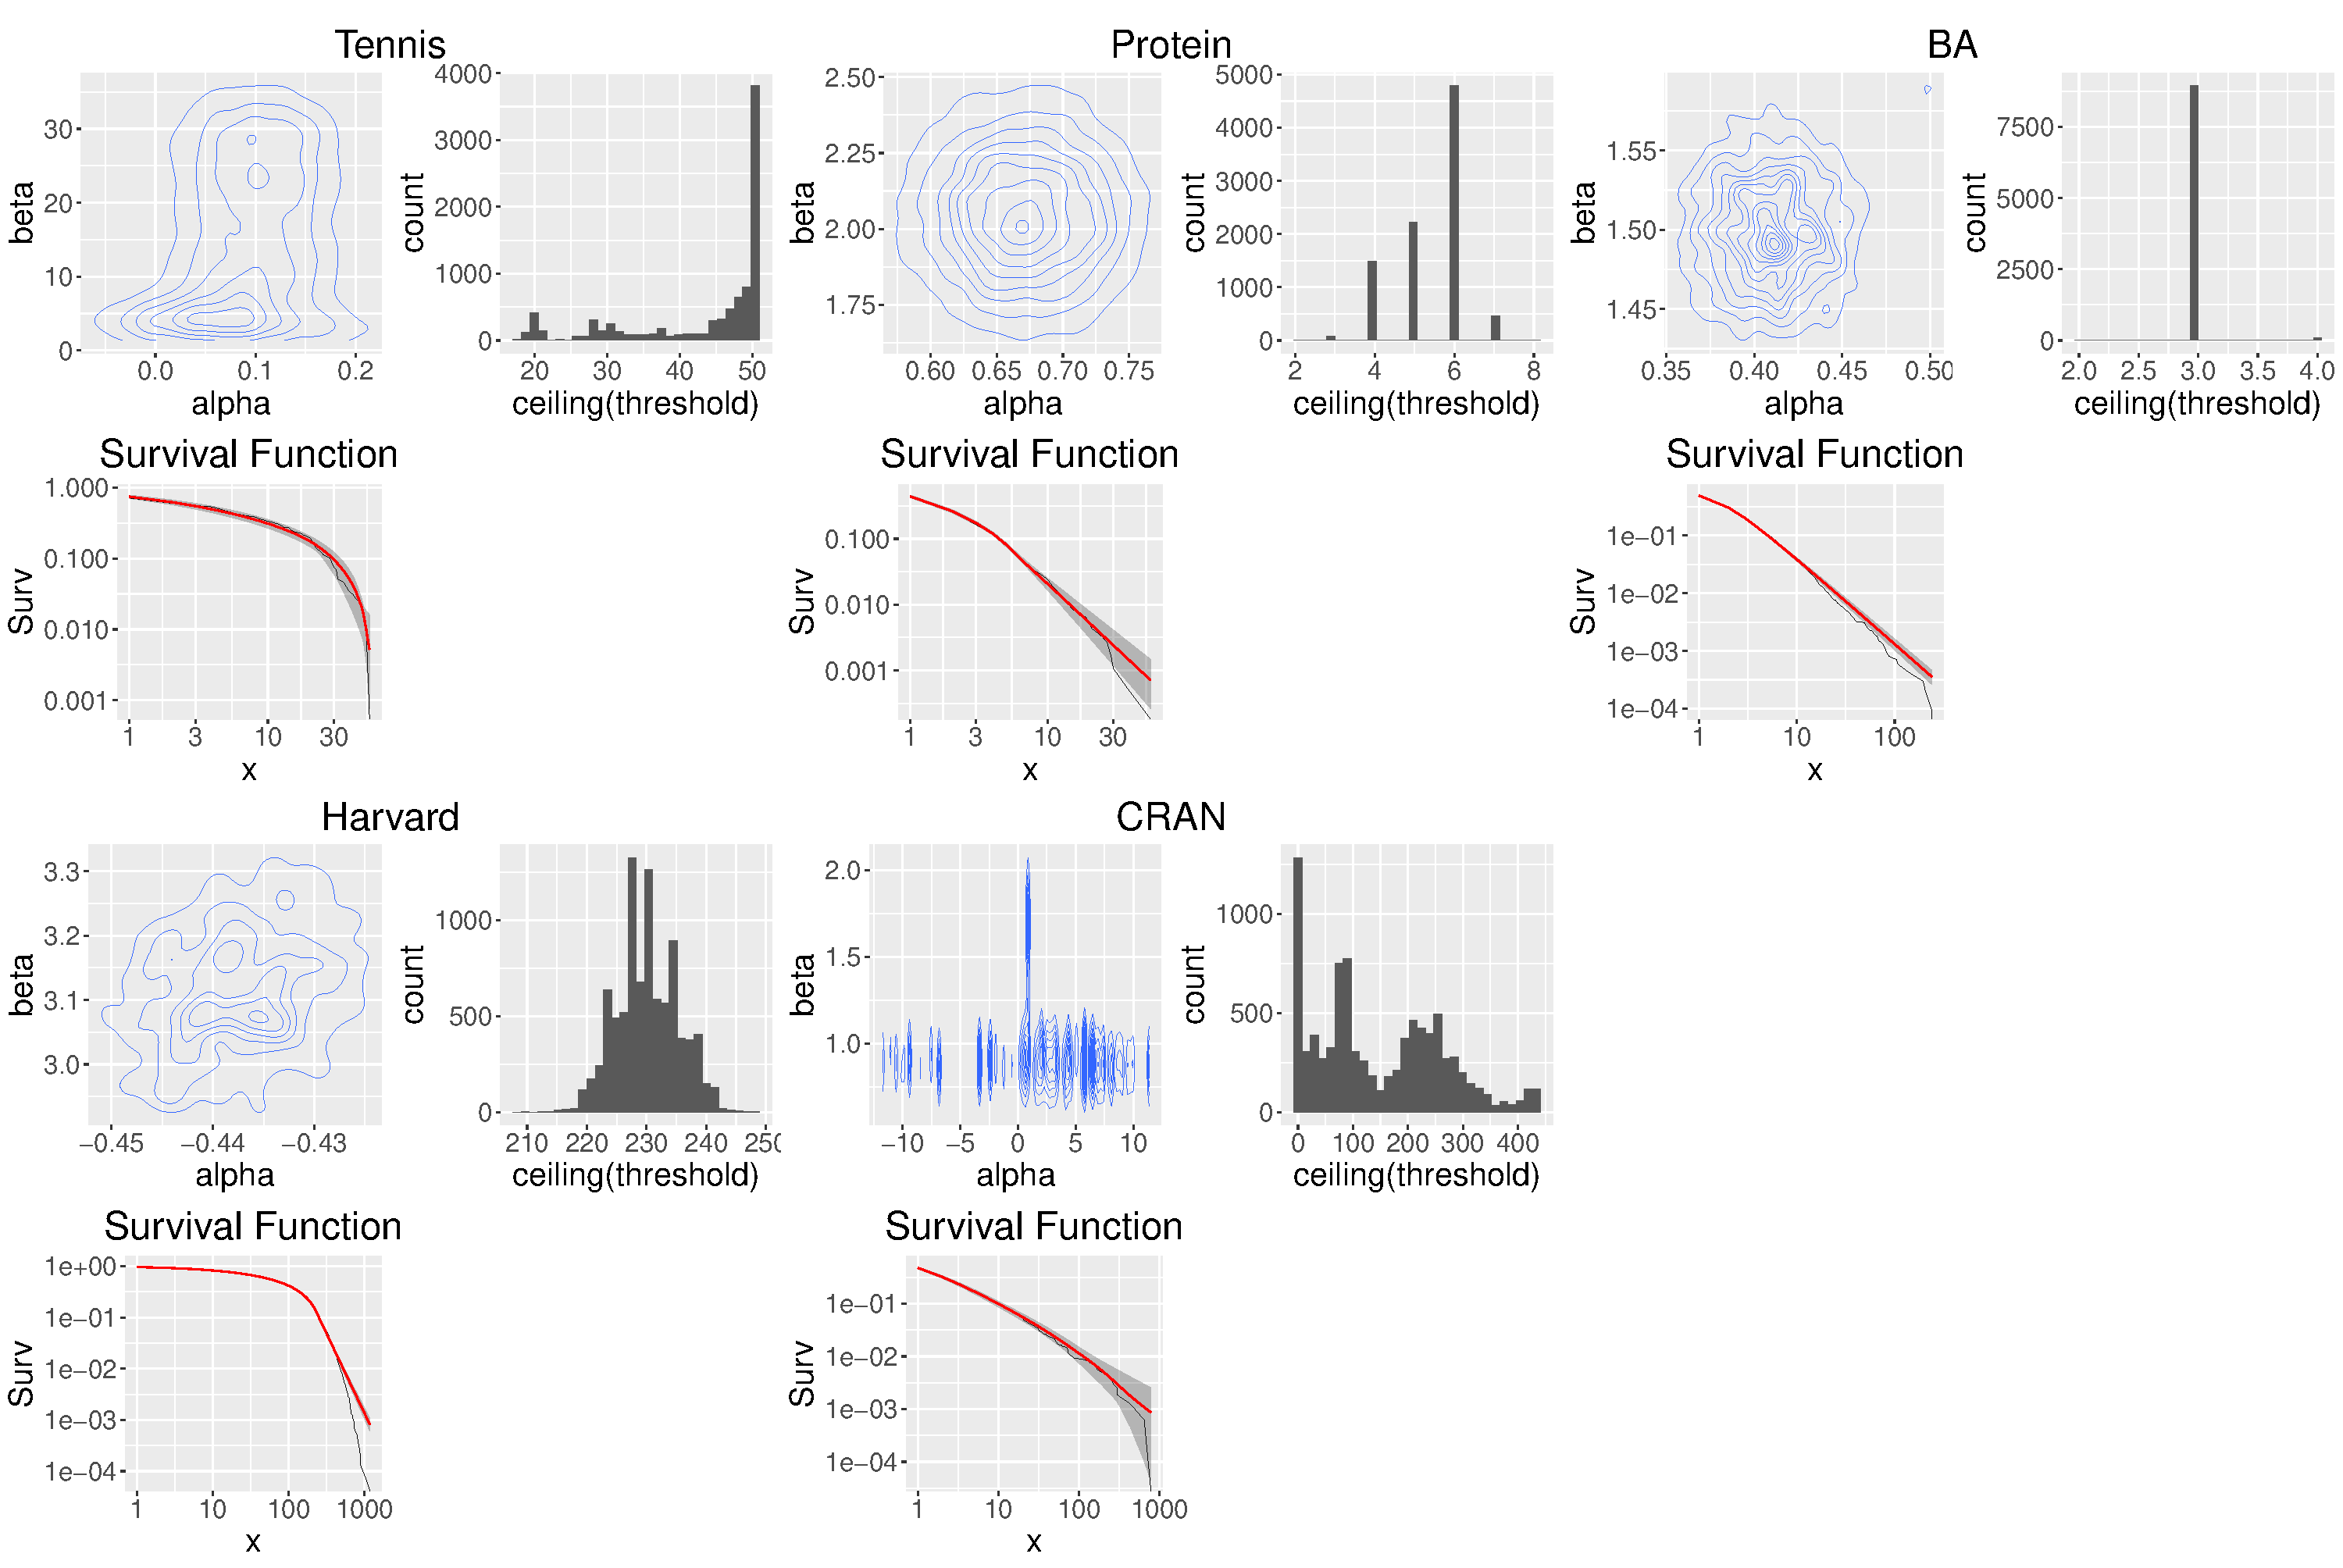
\includegraphics{proposal_files/figure-pdf/fig-plpl-1.pdf}

}

\caption{\label{fig-plpl}Fitted survival functions and posterior
densities of parameters.}

\end{figure}%

\subsubsection{Summary}\label{summary}

So far we have shown that the power law is only adequate for certain
sets of data, like the BA model and CRAN data, and seems to not be
useful for modelling many other sets of data. Introducing the power law
IGP mixture improves the performance of the model across almost all of
the data sets but is a lot more complex. To compromise between the two
we also included a power law mixture model, which seems to have yielded
similar results to the power law IGP mixture while having less
parameters. This will need to be investigated in more depth because it
may end up being preferable due to it being less complex.

Upon further investigation and seeing how well these models fit to
various sets of data, we will either decide to use one of them, or
decide to look for an alternative model to use. Then we can begin moving
along two directions, in one we look at tracking the changes in
parameters of the chosen model over time for various real data sets as
well as data simulated from the BA model. This informs what we do on the
other, where we will be attempting to modify and/or extend the BA model
so that the new model will provide a degree distribution that follows
the chosen model and matches up with the changes in parameters over time
for the data sets.

\newpage{}

\section{Project Plan}\label{project-plan}

\subsection{Objectives and more specific
goals}\label{objectives-and-more-specific-goals}

\subsubsection*{Review proofs of properties and modifications of the
Barabási-Albert model (months
3-9)}\label{review-proofs-of-properties-and-modifications-of-the-barabuxe1si-albert-model-months-3-9}
\addcontentsline{toc}{subsubsection}{Review proofs of properties and
modifications of the Barabási-Albert model (months 3-9)}

This will involve mostly reading of the original papers detailing the
properties of the BA model, with some attempt to recreate the proofs
perhaps in a more mathematically rigorous fashion. This may also help in
future when it comes to deriving the properties of the new model. It
will also be useful to identify what has already been done to modify or
extend the BA model. Some of the papers already lined up to read are:

\begin{itemize}
\tightlist
\item
  Dorogovtsev, Mendes, and Samukhin (2000)
\item
  Barabási, Albert, and Jeong (1999)
\item
  Wang and Resnick (2022)
\end{itemize}

\subsubsection*{Read extreme value theory and network science materials
(months
6-12)}\label{read-extreme-value-theory-and-network-science-materials-months-6-12}
\addcontentsline{toc}{subsubsection}{Read extreme value theory and
network science materials (months 6-12)}

This will also involve mostly reading of materials that will help in
understanding the mathematics behind network generative models in
addition to some extreme value theory that will be needed when it comes
to properly defining the model we choose for degree distributions and
its properties.

\subsubsection*{Monitor changes in model parameters for various real
networks (months
18-24)}\label{monitor-changes-in-model-parameters-for-various-real-networks-months-18-24}
\addcontentsline{toc}{subsubsection}{Monitor changes in model parameters
for various real networks (months 18-24)}

This will be an ongoing process throughout some of the other steps, all
while using the results produced to inform how we carry out the other
steps.

\subsubsection*{Use these changes to inform modification of the BA model
(months
24-30)}\label{use-these-changes-to-inform-modification-of-the-ba-model-months-24-30}
\addcontentsline{toc}{subsubsection}{Use these changes to inform
modification of the BA model (months 24-30)}

We will begin investigating possible modifications to the BA model that
will produce a degree distribution that aligns with the chosen model and
hopefully with the changes in the model parameters over time as the
networks grow.

\subsubsection*{Investigate properties of the new model (months
30-36)}\label{investigate-properties-of-the-new-model-months-30-36}
\addcontentsline{toc}{subsubsection}{Investigate properties of the new
model (months 30-36)}

Once a set of modifications has been made, we will then study the
theoretical properties of networks that grow under the new model.

\subsection{Outcomes}\label{outcomes}

\subsubsection*{Develop a suitable model for the degree distribution
(\textasciitilde{} month
12)}\label{develop-a-suitable-model-for-the-degree-distribution-month-12}
\addcontentsline{toc}{subsubsection}{Develop a suitable model for the
degree distribution (\textasciitilde{} month 12)}

We want a model that is capable of modelling the degree distributions of
real networks, and the changes in them over time.

\subsubsection*{Create set of functions and/or R package to fit the
model (\textasciitilde{} month
18)}\label{create-set-of-functions-andor-r-package-to-fit-the-model-month-18}
\addcontentsline{toc}{subsubsection}{Create set of functions and/or R
package to fit the model (\textasciitilde{} month 18)}

After coming up with a suitable model, we will require a way to fit it
in a somewhat uninvolved process so that the model can be fit to many
sets of data over many time frames.

\subsubsection*{Develop modifications of the BA model (
\textasciitilde{} month
30)}\label{develop-modifications-of-the-ba-model-month-30}
\addcontentsline{toc}{subsubsection}{Develop modifications of the BA
model ( \textasciitilde{} month 30)}

We want to develop some new model, based on the BA model, that can more
accurately describe how real networks have grown.

\section{Training Needs}\label{training-needs}

As part of the project I will require some training, below is a list of
some I intend to undergo:

\begin{itemize}
\tightlist
\item
  C++
\item
  Using the HPC
\item
  Communication, presentation and public speaking Skills
\item
  Thesis writing
\end{itemize}

\section*{References}\label{references}
\addcontentsline{toc}{section}{References}

\phantomsection\label{refs}
\begin{CSLReferences}{1}{0}
\bibitem[\citeproctext]{ref-Barabasi99}
Barabási, Albert-László, and Réka Albert. 1999. {``Emergence of Scaling
in Random Networks.''} \emph{Science} 286 (5439): 509--12.
\url{https://doi.org/10.1126/science.286.5439.509}.

\bibitem[\citeproctext]{ref-BARABASI1999173}
Barabási, Albert-László, Réka Albert, and Hawoong Jeong. 1999.
{``Mean-Field Theory for Scale-Free Random Networks.''} \emph{Physica A:
Statistical Mechanics and Its Applications} 272 (1): 173--87.
https://doi.org/\url{https://doi.org/10.1016/S0378-4371(99)00291-5}.

\bibitem[\citeproctext]{ref-Broido_2019}
Broido, Anna D., and Aaron Clauset. 2019. {``Scale-Free Networks Are
Rare.''} \emph{Nature Communications} 10 (1).
\url{https://doi.org/10.1038/s41467-019-08746-5}.

\bibitem[\citeproctext]{ref-Dorogovtsev2000}
Dorogovtsev, Sergey, José Fernando Mendes, and A Samukhin. 2000.
{``Structure of Growing Networks with Preferential Linking.''}
\emph{Physical Review Letters} 85 (November): 4633--36.
\url{https://doi.org/10.1103/PhysRevLett.85.4633}.

\bibitem[\citeproctext]{ref-Gilbert59}
Gilbert, E. N. 1959. {``{Random Graphs}.''} \emph{The Annals of
Mathematical Statistics} 30 (4): 1141--44.
\url{https://doi.org/10.1214/aoms/1177706098}.

\bibitem[\citeproctext]{ref-2011HoMC}
\emph{Handbook of Markov Chain Monte Carlo}. 2011. Chapman \& Hall/CRC
Handbooks of Modern Statistical Methods.

\bibitem[\citeproctext]{ref-Rohrbeck_2018}
Rohrbeck, Christian, Emma F. Eastoe, Arnoldo Frigessi, and Jonathan A.
Tawn. 2018. {``{Extreme value modelling of water-related insurance
claims}.''} \emph{The Annals of Applied Statistics} 12 (1): 246--82.
\url{https://doi.org/10.1214/17-AOAS1081}.

\bibitem[\citeproctext]{ref-Voitalov_2019}
Voitalov, Ivan, Pim van der Hoorn, Remco Hofstad, and Dmitri Krioukov.
2019. {``Scale-Free Networks Well Done.''} \emph{Physical Review
Research} 1 (October).
\url{https://doi.org/10.1103/PhysRevResearch.1.033034}.

\bibitem[\citeproctext]{ref-wang2022random}
Wang, Tiandong, and Sidney Resnick. 2022. {``Random Networks with
Heterogeneous Reciprocity.''} \url{https://arxiv.org/abs/2208.00348}.

\bibitem[\citeproctext]{ref-XIANG2014240}
Xiang, Fei, and Peter Neal. 2014. {``Efficient MCMC for Temporal
Epidemics via Parameter Reduction.''} \emph{Computational Statistics \&
Data Analysis} 80: 240--50.
https://doi.org/\url{https://doi.org/10.1016/j.csda.2014.07.002}.

\end{CSLReferences}



\end{document}
